%\documentclass[11pt,titlepage,twoside]{article}
%%\usepackage[letterpaper,margin=1in]{geometry}
%\usepackage[letterpaper,
%  showcrop,
%  margin=.67in,
%  layoutsize={5.5in,8.5in},
%  layoutoffset={1.5in,1.25in}]{geometry}
%\usepackage{enumitem}
%\usepackage{tikz}
%\usepackage{amsmath}
%\usepackage{xcolor,colortbl}
%\usepackage{caption}
%\usepackage{subcaption}
%\usepackage{siunitx}
%
%\setlength{\parindent}{0pt}
%\setlength{\parskip}{8pt}
%
%\captionsetup{
%  width=.8\linewidth, % width of caption is 90% of current textwidth
%  labelfont=bf,        % the label, e.g. figure 12, is bold
%  font=footnotesize,   % the whole caption text (label + content) is small
%  format=hang,         % no caption text under the label
%}
%%\captionsetup[subfigure]{
%%  format=plain,   % but allowed in subfigure to save space
%%}
%
%\sisetup{
%  inter-unit-product=\cdot,
%  per-mode=symbol
%}
%
%\tikzset{
%  >=latex
%}
%\tikzstyle{every node}=[font=\footnotesize]
%\tikzstyle{axes}=[thick,->]
%\tikzstyle{vectors}=[ultra thick,->]
%\tikzstyle{mass}=[thick,fill=cyan!35]
%\tikzstyle{function}=[very thick,red!80!black]
%
%\usetikzlibrary{decorations.pathmorphing,patterns}



%\newtcolorbox{exercise}[1][]{
%  enhanced,
%  skin=enhancedlast jigsaw,
%  attach boxed title to top left={xshift=-4mm,yshift=-0.5mm},
%  fonttitle=\bfseries\sffamily,
%  colbacktitle=blue!50,
%  colframe=blue!60!gray,
%  interior style={
%    top color=blue!10,
%    bottom color=red!10
%  },
%  boxed title style={
%    empty,
%    arc=0pt,
%    outer arc=0pt,
%    boxrule=0pt
%  },
%  underlay boxed title={
%    \fill[blue!60!gray] 
%      (title.north west) -- 
%      (title.north east) -- 
%      +(\tcboxedtitleheight-1mm,-\tcboxedtitleheight+1mm) -- 
%      ([xshift=4mm,yshift=0.5mm]frame.north east) -- 
%      +(0mm,-1mm) -- 
%      (title.south west) -- cycle;
%    \fill[blue!45!white!50!black] 
%      ([yshift=-0.5mm]frame.north west) -- 
%      +(-0.4,0) -- 
%      +(0,-0.3) -- cycle;
%    \fill[blue!45!white!50!black] 
%      ([yshift=-0.5mm]frame.north east) -- 
%      +(0,-0.3) -- 
%      +(0.4,0) -- cycle; 
%  },
%  title={Exercise},
%  #1
%}

%\titleformat{\section}{\HUGE\normalfont}
%\titleformat*{\section}{\bfseries}
%\titlespacing\section{0pt}{10pt plus 4pt minus 2pt}{4pt plus 12pt minus 2pt}
%
%
\chapter{Advanced Graphing Techniques}
%\author{Timothy Leung}
%\date{\today}
%
%
%\begin{document}
%\maketitle

\section{Introduction}


\section{Plotting $x$ vs.\ $t^2$}
In an experiment, a toy cart rolls down a ramp from rest (i.e.\ $v_0=0$), as
shown in Figure~\ref{fig:cart1}. At regular distances, time is recorded. In
this case, the acceleration of the cart \emph{should} be constant. Can we
determine the car's acceleration?
\begin{figure}[ht]
  \centering
  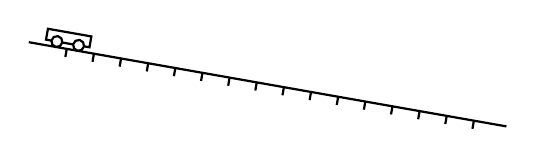
\begin{tikzpicture}[scale=.7,rotate around={-10:(9,0)}]
    \draw[thick] (0,0)--+(8.8,0);
    \draw[thick] (.3,.1) rectangle +(.8,.2);
    \draw[thick,fill=black!2] (.5,.1) circle (.1);
    \draw[thick,fill=black!2] (.9,.1) circle (.1);
    \foreach \x in {.7,1.2,...,8.5}
    \draw[thick](\x,0)--+(0,-.15); % node[below]{\tiny$\x$};
  \end{tikzpicture}
  \caption{Experimental set up for a toy cart rolling down a ramp}
  \label{fig:cart1}
\end{figure}

In such an experiment, we can generate a table of positions and the
corresponding time stamp when the cart is there, shown below:
\begin{center}
  \begin{tabular}{c|c}
    $x$ & $t$ \\\hline
    $x_0$ & 0 \\
    $x_1$ & $t_1$\\
    \vdots & \vdots \\
    $x_N$ & $t_N$
  \end{tabular}
\end{center}
%TML  \end{columns}
%TML  
%TML  \vspace{.3in}
%TML  \begin{columns}[T]
%TML    \column{.51\textwidth}
%TML    \uncover<2->{\color{magenta}
    
Based on the data, we can easily plot an $x$--$t$ graph.
\begin{figure}[ht]
  \centering
  \begin{tikzpicture}
    \draw[axes](0,0)--(0,2) node[right]{$x$};
    \draw[axes](0,0)--(2,0) node[right]{$t$};
    \draw[smooth,domain={0:1.8},very thick] plot(\x,{.4*\x*\x+.3});
  \end{tikzpicture}
\end{figure}
Since we expect acceleration to be uniform\footnote{i.e.\ constant}, the graph
should look like a parabola. Unfortunately this graph would not be very helpful
in determining acceleration. In general, in a position vs.\ time graph, it is
easy to get position, displacement and average velocity. However finding the
instantaneous velocity is very difficult, and finding the instantaneous
acceleration is nearly impossible.

We could, use a spreadsheet or statistics problem to fit a quadratic function
to the data, and then find the acceleration. However, in general, these
software packages will only give you what you ask for.

If, instead, we plot $x$--$t^2$, the graph would be \emph{linear}, and the
slope will tell us about the acceleration.
\begin{center}
  \begin{tabular}{c|c}
    $x$ & $t^2$ \\\hline
    $x_0$ & 0 \\
    $x_1$ & $t_1^2$\\
    \vdots & \vdots \\
    $x_N$ & $t_N^2$
  \end{tabular}
\end{center}
\begin{figure}[ht]
  \centering
  \begin{tikzpicture}
    \draw[axes] (0,0)--(0,2) node[right]{$x$};
    \draw[axes] (0,0)--(2,0) node[right]{$t^2$};
    \draw[very thick] (0,.3)--(1.8,1.8);
  \end{tikzpicture}
\end{figure}
When we plot $x$ as a function of $t^2$ instead of a function of $t$, we are
essentially doing this to the kinematic equation (from a few slide ago):
\begin{displaymath}
  \underbrace{x}_y=\underbrace{x_0}_b +
  \underbrace{\frac12a}_m\underbrace{t^2}_x
\end{displaymath}
and turning it into a linear function in the form $y=mx+x$ that is familiar to
everyone.
\begin{itemize}
\item The slope of the $x$ vs. $t^2$ graph is $\dfrac12a$ (or acceleration
  is 2 times the slope)
\item If the $x$ vs.\ $t^2$ graph is \emph{not} linear, we will know that
  our assumption of constant acceleration was incorrect, and that there are
    other factors that we neglected
\end{itemize}


\section{Plotting $v^2$ vs.\ $\Delta x$}

\begin{figure}[ht]
  \centering
  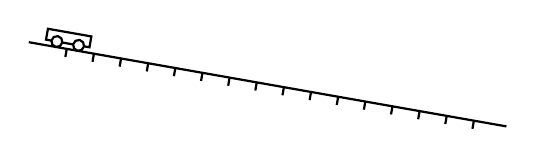
\begin{tikzpicture}[scale=.7,rotate around={-10:(9,0)}]
    \draw[thick] (0,0)--+(8.8,0);
    \draw[thick] (.3,.1) rectangle +(.8,.2);
    \draw[thick,fill=black!2] (.5,.1) circle (.1);
    \draw[thick,fill=black!2] (.9,.1) circle (.1);
    \foreach \x in {.7,1.2,...,8.5}
    \draw[thick](\x,0)--+(0,-.15); % node[below]{\tiny$\x$};
  \end{tikzpicture}
\end{figure}
A toy cart rolls down a ramp. At regular positions $x$ along the ramp, the
cart's velocity $v$ is recorded instead. Again, acceleration \emph{should}
be constant. Can we determine the car's acceleration from the data?

Plotting the data would give us a $v$--$x$ graph. Unfortunately (again) this
graph would not help us find the acceleration.
%TML
%TML      \begin{tabular}{c|c}
%TML        $x$ & $v$ \\\hline
%TML        $x_0$ & $v_0$ \\
%TML        $x_1$ & $v_1$\\
%TML        \vdots & \vdots \\
%TML        $x_N$ & $v_N$
%TML      \end{tabular}
%TML      \hspace{.2in}
%TML      \begin{minipage}{.6\textwidth}
\begin{figure}[ht]
  \centering
  \begin{tikzpicture}
    \draw[axes] (0,0)--(0,2) node[right]{$v$};
    \draw[axes] (0,0)--(2,0) node[right]{$x$};
    \draw[smooth,domain={0:1.8},samples=40,very thick]
    plot(\x,{\x^.5+.3});
  \end{tikzpicture}
\end{figure}

But if we plot $v^2$ vs.\ $\Delta x$, the graph would be \emph{linear},
and the slope will give us information about acceleration.

%TML      \begin{tabular}{c|c}
%TML        $v^2$ & $\Delta x$ \\\hline
%TML        $v_0$ & 0 \\
%TML        $v_1$ & $x_1-x_0$\\
%TML        \vdots & \vdots \\
%TML        $v_N$ & $x_N-x_0$
%TML      \end{tabular}
%TML      \hspace{.2in}
\begin{figure}[ht]
  \centering
  \begin{tikzpicture}
    \draw[axes] (0,0)--(0,2) node[right]{$v^2$};
    \draw[axes] (0,0)--(2,0) node[right]{$\Delta x$};
    \draw[very thick] (0,.3)--(1.8,1.8);
  \end{tikzpicture}
\end{figure}

If velocity and position are given, then the relationship would be best
expressed using this kinematic equation (we have studied a few slide ago):

\begin{displaymath}
  \underbrace{v^2}_y=\underbrace{v_0^2}_b+\underbrace{2a}_m
  \underbrace{(x-x_0)}_x
\end{displaymath}

by plotting $v^2$ vs. $\Delta x=x-x_0$, we again have a linear function in the
form of $y=mx+b$.
\begin{itemize}
\item The slope of the graph is two times the acceleration $m=2a$ (i.e.\
  acceleration is one half of the slope).
\item The square of the initial velocity ($v_0^2$) is the $y$-intercept
\item \emph{If} our assumption was incorrect (i.e.\ acceleration is \emph{not}
  constant) then the line would not be straight
\end{itemize}


\section{Graphing Other ``Linear'' Functions}
This concept of turning non-linear relationships into linear graphs by
tranposing variables also extends to graphing other physical relationships not
related to kinematics.

\subsection{Finding Index of Refraction}
For example, when light is refracted into another medium, as shown in
Fig.~\ref{fig:snell},
\begin{figure}[ht]
  \centering
  \begin{tikzpicture}
    \fill[lightgray] (-3,-2) rectangle (3,0);
    \draw[thick] (-3,0)--(3,0);
    \draw[red,very thick] (-2,2)--(0,0)--(1,-2)
    node[below,black]{Refraction};
    \draw[red,very thick] (0,0)--(2,2) node[right=0,black]{Reflection};
    \draw[dashed] (0,2)--(0,-2);
    \draw[axes] (0,1) arc (90:135:1) node[midway,above]{$\theta_1$};
    \draw[axes] (0,-1) arc (270:297:1) node[midway,below]{$\theta_2$};
    \node[above] at (-2,0) {$n_1$};
    \node[below] at (-2,0) {$n_2$};
  \end{tikzpicture}
  \caption{Refraction of light into another medium}
  \label{fig:snell}
\end{figure}
the relationship between the incident angle $\theta_1$ and the refracted angle
$\theta_2$ is given by \textbf{Snell's law}, also known as the
\textbf{law of refraction}:
\begin{equation}
  n_1\sin\theta_1=n_2\sin\theta_2
\end{equation}
To experimentally find the index of refraction of one of the media (e.g.\
$n_2$), we can vary the incident angle $\theta_1$ in a medium with a known
index of refraction $n_1$, and measure the resulting refracted angle $\theta_2$.
However, simplying plotting $\theta_1$ vs.\ $\theta_2$ will result in a graph
shown in Figure~\ref{fig:snell2}. The graph does not easily give you
information about $n_2$.
\begin{figure}
  \centering
  \begin{tikzpicture}[scale=2]
    \draw[axes] (0,0)--+(1.8,0) node[right]{$\theta_1$};
    \draw[axes] (0,0)--+(0,1.5) node[right]{$\theta_2$};
    \draw[smooth,domain={0:1.55},very thick] plot(\x,{asin(sin(60*\x)/1.3)/60});
    \draw[dotted] (0,0)--(1.5,1.5);
  \end{tikzpicture}
  \caption{Plotting $\theta_1$ vs.\ $\theta_2$ in a refraction problem}
  \label{fig:snell2}
\end{figure}
However, if we plot $\sin\theta_1$ vs.\ $\sin\theta_2$, i.e.:
\begin{equation*}
  \underbrace{\sin\theta_2}_y=\underbrace{\left[\frac{n_1}{n_2}\right]}_m
  \underbrace{\sin\theta_1}_x
\end{equation*}
Then the slope is the ratio of the indices $n_1/n_2$.
%In an experiment, we can vary the incident angle $\theta_1$ in a medium with a
%known index ($n_1$), and measure the corresponding refracted angle $\theta_2$.
%Once the slope of the graph ($n_1/n_2$) is known, we can find $n_2$.

\subsection{Finding $g$ Using Simple Pendulums}

To relate the period of oscillation (the time it takes to swing back and
forth once) of a simple pendulum to the length of the pendulum, plot $T$
vs.\ $\sqrt\ell$:

\begin{equation*}
  \underbrace{T}_y=\underbrace{\frac{2\pi}{\sqrt g}}_m
  \underbrace{\sqrt\ell}_x
\end{equation*}

or alternatively, by squaring both sides of the equation to relate $T^2$ to
$\ell$:
\begin{equation*}
  \underbrace{T^2}_y=\underbrace{\left[\frac{4\pi^2}g\right]}_m
  \underbrace{\ell}_x
\end{equation*}
We can change the length of the pendulum $\ell$ and measure the period $T$ of
the oscillation. This relationship will be studied in the last topic of this
course, in Class 15
%TML\end{frame}
%TML
%TML
%TML
%TML\section{Acceleration due to Gravity}
%TML
%TML\begin{frame}{Acceleration Due to Gravity}
%TML  \begin{columns}
%TML    \column{.4\textwidth}
%TML    \pic{1.1}{pisa}
%TML    
%TML    \column{.6\textwidth}
%TML    \begin{itemize}
%TML    \item Before Galileo people thought that heavier objects falls faster than
%TML      lighter objects
%TML    \item Galileo, a mathematics professor at the University of Pisa,
%TML      supposedly dropped two cannonballs of different masses from the Tower of
%TML      Pisa; they hit the ground at the same time
%TML    \end{itemize}
%TML  \end{columns}
%TML\end{frame}
%TML
%TML
%TML
%TML\begin{frame}{Acceleration Due to Gravity}
%TML  Acceleration due to the gravitational attraction between the object and Earth
%TML  is constant near the surface of Earth, with a magnitude of
%TML  
%TML  \eq{-.1in}{
%TML    \boxed{
%TML      g=\SI{9.81}{\metre\per\second\squared}
%TML    }
%TML  }    
%TML  \begin{itemize}
%TML  \item Always points down
%TML  \item Constant regardless of whether the object is being drop, or being
%TML    thrown upwards, down or sideways
%TML  \item Constant regardless of the mass of the object
%TML  \item The value differs slightly at different parts on Earth
%TML  \item In AP Physics, you can use
%TML    $\boxed{g=\SI{10}{\metre\per\second\squared}}$ in your calculations
%TML  \end{itemize}
%TML\end{frame}
%TML
%TML
%TML
%TML\begin{frame}{Free Fall}
%TML  A free-falling object is one that is falling under the sole influence of
%TML  gravity
%TML  \begin{itemize}
%TML  \item i.e.\ acted only by the force of gravity
%TML  \item Almost \emph{all} moving objects on Earth are also subjected to air
%TML    resistance, so strictly speaking, \emph{nothing} is in a real free-fall.
%TML  \item Luckily, in AP Physics, we will be ignoring air resistance for the
%TML    most part
%TML  \end{itemize}
%TML  Examples:
%TML  \begin{itemize}
%TML  \item A baseball that is thrown
%TML  \item A skydiver just after jumping out of an airplane
%TML  \item A bullet fired from a gun
%TML  \item The International Space Station
%TML  \end{itemize}
%TML\end{frame}
%TML
%TML
%TML
%TML\begin{frame}{Example Problem}
%TML  \textbf{Example:} I am standing on observation deck on the 86-th floor of the
%TML  Empire State Building in New York City, which is about \SI{320}{\metre} above
%TML  ground. I drop my phone onto Fifth Avenue below. Ignoring air resistance, how
%TML  long does take before my phone hit the pavement below? At what velocity?
%TML  
%TML  \vspace{1in}This problem is obviously completely unrealistic, because the
%TML  effects of air resistance is \emph{very} significant.
%TML\end{frame}
%TML
%TML\end{document}



%\newcommand{\pic}[2]{\includegraphics[width=#1\textwidth]{#2}}


%
%
%
%
%e}
%y my lecture notes plus the slides for Grade 11 Physics, Grade
%P Physics 1.
%
% this booklet are usually presented over two $2\frac12$-hour
%h my Grade 11 and AP Physics 1 classes, and one $2\frac12$-hour
%classes as a review.
%
%
%
%
%
%
%}
%aphics/worldslongestroadtrainwithpowertrailer8}
%
%
%s are connected by a cable or a solid linkage with negligible
%
%s (usually) have the same acceleration
%ltiple free-body diagrams
%
%
%
%ction}
%-body problem, you can follow these procedures:
%}
% on each of the objects
%e forces on all the objects along the direction of motion
%}
%n of motion is usually very obvious
%ternal forces should cancel and do not figure into the
%on of the system
%
%e acceleration of the entire system using second law of motion
%}
% that (usually) every object has the same acceleration!
%
% the FBD of each of the objects and compute the unknown
%
%
%
%Along Level Surfaces}
%
%cts Connected by Massless Cables}
%_1$, $m_2$ and $m_3$) are connected by massless
%Obviously cables are not \emph{literally} massless, but here,
%he masses of the cables are insignificant compared to the
%efore we can ignore them without making our answers
% pulled to the right by an external force $\vec F$ across a
%s shown in Figure~\ref{fig:tension}. The coefficient of kinetic
% the masses and the surface is $\mu$.
%t]
%
%ture}
% (0,0)--(10,0);
%(1,0) rectangle (2.5,1) node[midway]{$m_3$};
%line width=2] (2.5,.5)--(4,.5)
%above]{$T_2$};
%(4,0) rectangle (5.5,1) node[midway]{$m_2$};
%line width=2] (5.5,.5)--(7,.5)
%above]{$T_1$};
%(7,0) rectangle (8.5,1) node[midway]{$m_1$};
%s] (8.5,.5)--(9.3,.5) node[right]{$\vec F$};
%re}
% masses are connected by massless cables and accelerate
%
%sion}
%
%
%, we want to consider the following questions:
%}[nosep,leftmargin=15pt]
%he forces acting on each of the masses?
%e acceleration of the system, assuming that the cables do not
%
%he magnitudes of the tension forces ($T_1$ and $T_2$) in the
%
%
%
%-Free-Body Diagrams:} Our first step to finding the solution to
% to draw free-body diagrams for each of the masses, as shown in
%fbd1}.
%t]
%
%ture}[lightgray]
%-(9.5,0);
%rectangle (2.5,1) node[midway]{$m_3$};
%idth=2] (2.5,.5)--(4,.5);
%rectangle (5.5,1) node[midway]{$m_2$};
%idth=2] (5.5,.5)--(7,.5);
%rectangle (8.5,1) node[midway]{$m_1$};
%}[vectors]
%pe}[orange]
%.75,.5) circle (.1);
%.75,.5)--(1.75,-1) node[below]{$m_3\vec g$};
%(1.75,.5)--(1.75,2) node[above]{$\vec N_3$};
%(1.75,.5)--(3,.5) node[above]{$\vec T_2$};
%(1.75,.5)--(1,.5) node[below]{$\vec f_3$};
%}
%pe}[violet]
%.75,.5) circle (.1);
%.75,.5)--(4.75,-1) node[below]{$m_2\vec g$};
%.75,.5)--(4.75,2) node[above]{$\vec N_2$};
%.75,.5)--(6,.5) node[above]{$\vec T_1$};
%.75,.54)--(3.5,.54) node[above]{$\vec T_2$};
%.75,.46)--(4,.46) node[below]{$\vec f_2$};
%}
%pe}[blue]
%.75,.5) circle (.1);
%.75,.5)--(7.75,-1) node[below]{$m_1\vec g$};
%.75,.5)--(7.75,2) node[above]{$\vec N_1$};
%.75,.5)--(9.75,.5) node[right]{$\vec F$};
%.75,.54)--(6.5,.54) node[above]{$\vec T_1$};
%.75,.46)--(7,.46) node[below]{$\vec f_1$};
%}
%
%re}
%body diagrams}
%1}
%
%
%note that
%nosep,leftmargin=15pt]
%orce $\vec F$ is only applied to $m_1$, therefore it
%ear on the other free-body diagrams
%iction of the masses are: $f_1=\mu N_1=\mu m_1g$,
%mu m_2g$, and $f_3=\mu N_3=\mu m_3g$. (In a general problem, the
%f friction do not need to be the same for all the masses, but
%ying the problem here.
%$T_2$ are action-reaction pair of forces
%
%
%
%-Second law of motion:} Once the free-body diagrams are
%n sum the forces along the direction of motion for each object,
%he second law of motion individually on each object.
%
%F-\mu m_1g-T_1} &= {\color{blue}m_1a}\label{eq:m1}\\
%} T_1-\mu m_2g-T_2} &= {\color{orange}m_2a}\label{eq:m2}\\
%} T_2-\mu m_3g} &= {\color{violet}m_3a}\label{eq:m3}
%
% do not break, all three masses have the same acceleration $a$
%t. Therefore we can \emph{sum} the three equations above
%}--\ref{eq:m3}) to get the expression:
%
%
%m_3)g &= (m_1+m_2+m_3)a\\
% \label{eq:law2-system}
%
%e second law of motion applied to the whole system as a single
% introduce the variable $M=m_1+m_2+m_3$ to represent the total
%e system.
%
%q.~\ref{eq:law2-system} to calculate the acceleration of the
%
%
% g
%l}
%
% problem, you may be solving for the algebraic expression, or
%cal value.
%
%-Unknown Forces:} Once the acceleration of the system is known,
%the other unknown forces---in this case, tension forces $T_1$
%
%
%is to solve for $T_2$ is to look at the force balance of
%_3$ (Eq.~\ref{eq:m3}). Solving for $T_2$ and substituting the
%t we got from Eq.~\ref{eq:accel}, we get:
%
% m_3 g\\
%red}a}+\mu g)\\
%olor{red}\frac FM-\mu g}+\mu g\right)\\
%F\\
%3}{m_1+m_2+m_3} F
%
%or $T_1$, we can use the force balance of $\color{blue}m_1$ in
% Solving for $T_1$, and substituting the acceleration from
%l}, we find the expression for $T_1$:
%
%color{red}a}+\mu g)\\
%\color{red}\frac FM-\mu g}+\mu g\right)\\
%M\\
%MF\\
%ac{m_2+m_3}{m_1+m_2+m_3}\right)F
%
%n also use the force balance of $\color{violet}m_2$ to find
%or $T_1$ in Eq.~\ref{eq:m2}:
%
%u m_2g + m_2a\\
%+ \mu g)\\
% + m_2\left(\frac FM -\mu g + \mu g\right)\\
%3}MF\\
%m_2+m_3}{m_1+m_2+m_3}\right)F\\
%
%e as before.
%
% another way to find $T_1$! This time we treat
%_2$ and $\color{orange}m_3$ as a single object. In this case, we add Eqs.~\ref{eq:m2} and \ref{eq:m3} together, and then solving for $T_1$
% acceleration from Eq.~\ref{eq:accel}:
%
%)(a+\mu g)\\
%frac FM-\mu g+\mu g)\\
%_3}MF\\
%_3}{m_1+m_2+m_3}F\\
%
%isingly, is the same answer as using the other two methods.
%multi-problem is an exercise that you have done many times
%sses: solving multiple equations with multiple unknowns. In
% are 3 unknowns ($a$, $T_1$ and $T_2$) and 3 equations.
%
%
%her Connected Bodies Example}
%$ and $m_2$) are being pushed along a level surface by an
% force $\vec F$, as shown in Figure~\ref{fig:pushed}. The
%inetic friction between the masses and the surface is $\mu$.
%s example, we want to consider the following questions:
%}[nosep,leftmargin=15pt]
%e acceleration of the masses?
%e normal force that $m_1$ exerts on $m_2$?
%
%very similar to the previous example.
%
%t]
%
%ture}[scale=4/3]
% (-1.5,0)--(3.5,0);
%rectangle (1,1) node[midway]{$m_1$};
%(1,0) rectangle (2.5,1.25) node[midway]{$m_2$};
%s] (-1,.5)--(0,.5) node[pos=0,left]{$\vec F$};
%re}
%asses pushed together by an external force}
%hed}
%
%
%-Free-body diagrams:} Like the previous problem, we start with
%y diagrams for each of the masses, shown in
%fbd-pushed}.
%t]
%
%re}{.4\textwidth}
%
%icture}[scale=4/3,orange,vectors]
%le (.07);
%)--+(1.4,0) node[right]{$\vec F$};
%)--+(0,-1) node[right]{$m_1\vec g$};
%)--+(0,1) node[left]{$\vec N_1$};
%05)--+(-.8,0) node[above]{$\vec N_{12}$};
%)--+(-.5,0) node[below]{$\vec f_1$};
%ture}
%Mass $m_1$}
%}
%re}{.4\textwidth}
%
%icture}[scale=4/3,vectors,violet]
%le (.07);
%)--+(0,1) node[right]{$\vec N_2$};
%)--+(-.45,0) node[below]{$\vec f_2$};
%)--+(0,-1) node[right]{$m_2\vec g$};
%)--+(.8,0) node[right]{$\vec N_{12}$};
%ture}
%Mass $m_2$}
%}
%body diagrams for the pushed-blocks example}
%-pushed}
%
%
%details about the normal forces.
%nosep,leftmargin=15pt]
% forces ($N_1$, $N_2$ and $N_{12}$) appear in the free-body
% they only act on the centre of mass. In fact, the normal force
% the entire contact surface.
% force $\vec N_{12}$ is at the contact between the two masses.
%n-reaction pair, similar to the tension force in the previous
%$m_1$ pushes against $m_2$ (action), $m_2$ pushes back against
%n).
%
%
%
%Second law of motion:} Using the free-body digrams, we then sum
% direction of motion for each mass:
%
%}F-N_{21}-\underbrace{\mu m_1g}_{f_1}} &={\color{orange}m_1a} \\
%}N_{12}-\underbrace{\mu m_2g}_{f_2}} &= {\color{violet}m_2a}
%
%ize that both masses must have the acceleration. Adding them
%e
%
%
%2)g  &= (m_1+m_2)a\\
% Ma \label{eq:system}
%
%$ is the total mass of the system of objects.
%em} is essentially the second law of motion applied to the
% if it is a single object. Solving for acceleration, we have:
%
%mu g
%l2}
%
%l2} is identical to Eq.~\ref{eq:accel} from our first example.
%last problem, acceleration can be expressed as an algebraic
%th numerical values depending on the problem.
%
%Find remaining forces:} Once acceleration is known, we can find
%known force: the normal force $N_{12}$ between the blocks.
% the normal force $N_{12}$ can be calculated using the
%uations of either mass. Using the equation for $M_1$ and solving
%
%
%_1({\color{red}a}+\mu g)\\
%e}F} - m_1\left({\color{red}\frac FM-\mu g} +\mu g\right) \\
%e}M\frac FM} - m_1\left(\frac FM\right) \\
%}M F\\
%{m_2}{m_1+m_2} F
%
%the same procedure to the force balance for $m_2$:
%
%({\color{red}a} + \mu g) \\
%\color{red}\frac FM-\mu g} + \mu g\right) \\
%frac FM\right) \\
%m_1+m_2} F
%
%e as before.
%
%
%ked Objects}
%$ and $m_2$) are stacked on top of each other above a
%le, as shown in Figure~\ref{fig:stacked}. An external force
%ied to $m_2$, causing both blocks to accelerate to the right
% slipping. The coefficients of static and kinetic friction
%es are $\mu_s$ and $\mu_k$ respectively.
%t]
%
%ture}
% (-1,0)--(5.5,0);
%rectangle (3,1) node[midway]{$m_2$};
%(.75,1) rectangle (2.25,1.75) node[midway]{$m_1$};
%s] (3,.5)--(4.5,.5) node[right]{$\vec F$};
%re}
%asses stacked on top of each other on a frictionless table.}
%cked}
%
%
%der the following questions:
%}[nosep,leftmargin=12pt]
%e maximum acceleration of the masses without slipping?
%e magnitude of the external force $F$ at maximum
%
%e acceleration of $m_1$ if $F$ exceeds this maximum value?
%
%
%
%Free-body diagrams:} As in the previous example, we draw
%ms of both masses.
%t]
%
%re}{.4\textwidth}
%
%icture}[orange,vectors]
%,1.375) circle (.1);
%,1.375)--+(1.5,0) node[right,fill=yellow!30]{$\vec f$};
%,1.375)--+(0,-1.2) node[right]{$m_1\vec g$};
%,1.375)--+(0,1.2)  node[left=3,fill=pink!20]{$\vec N_{12}$};
%ture}
%}
%re}{.4\textwidth}
%
%icture}[vectors,violet]
%,.5) circle (.1);
%,.5)--+(2,0) node[right]{$\vec F$};
%,.5)--+(-1.5,0) node[left,fill=yellow!30]{$\vec f$};
%5,.5)--+(0,-1.2) node[right]{$m_2\vec g$};
%5,.5)--+(0,-1.2) node[left=3,fill=pink!20]{$\vec N_{12}$};
%,.5)--+(0,1.2) node[left]{$\vec N_2$};
%ture}
%}
%
%tion-reaction pairs of forces:
%
%ce $N_{12}$ at the interface between $m_1$ and $m_2$ acts upwards
%ownwards on $m_2$
%ction\footnote{That is, if the blocks don't slide against each
%o, then the friction would be kinetic friction instead} $f$,
%terface between $m_1$ and $m_2$, acts forward on $m_1$, and
%m_2$.
%
% that actually accelerates $m_1$ forward! (Think about
%n there is no friction between the masses.)
%
%
% For problems like this, we focus on the top blocks first.
%ulls the block forward is the static friction force $f_s$.
%f motion applied to $m_1$ is:
%
%s}
%\textwidth}
%
%picture}[scale=.95,vectors,orange]
%cle (.08);
%0)--(1.5,0) node[right]{$\vec f_s$};
%0)--(0,-1.2) node[right]{$m_1\vec g$};
%0)--(0,1.2) node[left]{$\vec N_{12}$};
%cture}
%
%es along the direction of motion:
%
%
%
%tion $a_\text{max}$ occurs when static friction is also at
%f=\max f_s=\mu_s N_{12}=\mu_s m_1g$:
%
%
%m_1a_\text{max}\\
%=\mu_s g
%
%maximum acceleration is, in fact, independent of mass.
%
% Once the $a_\text{max}$ is known, we can use it to calculate
%ied force. We can do this by substituting the expression for
% the force balance for $m_2$:
%
%_\text{max}-f &= m_2a_\text{max}\\
%= m_2a_\text{max}+f_s\\
%+\mu_s m_1g\\
%=\mu_s(m_1+m_2)g
%
%le system as a single object with total mass of $m_1+m_2$:
%
%
%= (m_1+m_2)a_\text{max}\\
%_2)g
%
%ays gives you the same answer.
%
%Machine--Pulley Problems}
%
%ple Problem: Atwood Machine}
%d machine} is made of two objects connected by a rope that
%ey. The pulley allows the direction of force and direction
%nge between two objects.
%s}
%\textwidth}
%er}
%phics/pulley_prob_2}
%}
%\textwidth}
%mple:} The object on the left has a mass of $M$ and the object
%t has a mass of $m$.
%ize}
%is the acceleration of the masses?
%is the tension in the rope?
%e}
%
%
%
%y, an Atwood machine problem is one where two objects are
%surface. These surfaces may have (or may not) have friction. In
% two blocks are connected by a massless string over a
%pulley as shown in the diagram.
%t]
%
%ture}[scale=1.5,thick]
%thick,brown] (-2,.4)--(.1,.4);
%-(-4,0) node[pos=.35,below]{$\mu$};
%agenta!50] (-2,0) rectangle +(-1,.75) node[midway]{$m$};
%}[rotate=-30]
%a thick,brown] (1,.4)--(-.05,.4);
%)--(3,0) node[midway,below left]{$\mu$};
%] (1,0) rectangle (2.5,1) node[midway,rotate=-30]{$M$};
%
%}[rotate=-15]
%=gray] (0,.3) circle (.15);
%=lightgray] (0,.3) circle (.1);
%a thick] (0,0)--(0,.3);
%3) circle (.04);
%}
%(0,0)--(0,-1.5);
%,-.5) arc(270:330:.5) node[midway,below]{$\phi$};
%re}
%
%ate}[(a)]
%ne the acceleration of the blocks.
%te the tension in the string.
%e}
%\end{document}
